%!TEX root = ../main.tex
% !TeX encoding = UTF-8
\section{Experimentos}

    \subsection{Capacete para Segurança de Ciclistas}
        Desenvolveu-se um protótipo de capacete na qual realiza-se verificações de distância de objetos nas costas do ciclista a fim de alertá-lo de possíveis riscos de acidentes.
        Caso esteja em situação de risco, o capacete emitirá sinais visuais luminosos, além do envio de aviso para um segundo dispositivo, como um \textit{smartphone} avisando de sua situação.
        Construiu-se um capacete modular a fim de fazer análises com diferentes protótipos de leitura no capacete sendo este com 1 à 3 sensores de distância, além de um \buffer\ de dados de tamanho 5, 10 e 15 para processamento das distâncias de cada sensor, discutidos a seguir.
        Além da avaliação de performance e gasto energético, é possível ter diferentes precisões de distância com tais variações.
        
        \begin{figure}[h] \centering
            \vspace{-0.5em}
            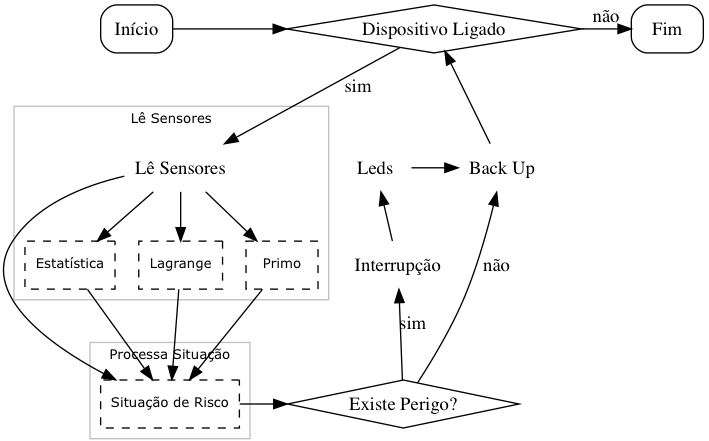
\includegraphics[width=0.48\textwidth]{img/capacete.png}
            \caption{Grafo de chamada do algoritmo base do \wearable. Itens quadriculados exibem a localização dos algoritmos candidatos ao particionamento.}
            \label{fig:gc}
        \end{figure}
        
        Como é exibido na Figura \ref{fig:gc}, os passos básicos do \wearable\ constituem-se basicamente de leitura das distâncias, cálculo de risco e aviso ao usuário.
        O particionamento será avaliado em duas seções principais, sendo elas a de leitura e de processo de situações, constituindo de 4 situações diferentes de particionamento para análise (itens pontilhados na Figura \ref{fig:gc}).
        Na seção de leitura de sensores, serão adicionados: \textit{a)} algoritmo de análise estatística (Algoritmo \ref{alg:statistic}) na qual calculará valores de desvio padrão e variância dos valores no \buffer; \textit{b)} algoritmo de lagrange (Algoritmo \ref{alg:lagrange}) interpolará novas distâncias a partir dos dados do \buffer\ e; \textit{c)} algoritmo de números primos (Algoritmo \ref{alg:prime}) avaliará se a soma das distâncias lidas correspondem à números primos.
        A análise serão feitas por meio de exclusão, selecionando apenas um algoritmo por vez e adicionado ao código para análise.
        Quando nenhum desta seção for utilizado para particionamento, utiliza-se então: \textit{d)} algoritmo de processamento de risco (Algoritmo \ref{alg:risk}), na seção de processo de situações.
        Obrigatoriamente, este último estará em todas as análises mesmo quando não particionado, pois é passo necessário para a iteração do \wearable.
        Todos os códigos dos algoritmos particionados estão em anexo.
        
        %algos
    
        \subsubsection{Recursos Utilizados}
            A placa utilizada para sintetização foi uma Arty A7-35T com 32 mil \luts\ (LuTs) sem um \textit{hard-processor}, ou seja, um controlador/processador físico dedicado.
            Então, par isso, utilizou-se o sistema \textit{soft-processor} MicroBlaze para processamento do código em \software.
            Todos os algoritmos foram construídos utilizando ferramenta de HLS e incorporados ao projeto base com construções de circuitos digitais assistidos pelo computador.
            A comunicação entre \hs\ é feita utilizando interface AXI.
            A medição de distância é realizada com um sensor ultrassônico e a comunicação com o segundo dispositivo utiliza \textit{Bluetooth Low Energy}.
        
        
    \subsection{Testes Realizados}
        % Explicando os testes
        Para a realização dos testes, foi feito um procedimento tendo base a Figura \ref{fig:distance}. 
        
        \begin{figure}[h] \centering
            %\vspace{-0.5em}
            
\includegraphics[width=0.5\textwidth]{img/distance.png}
            \caption{Simulação de aproximações de objetos perante o ciclista segundo suas respectivas áreas de segurança.}
            \label{fig:distance}
        \end{figure}
    
        Cada experimento será realizado no decorrer de 12 iterações\footnote{Iteração denominada como um ciclo completo de leitura, processamento e atuação do \wearable}. 
        Os principais passos do teste são:
        \begin{itemize}
            \item 
            %
            \textit{Iteração 1:} o ciclista encontra-se a uma distância de 130 centímetros do objeto, sendo sua situação declarada como Segura;
            %
            \item 
            \textit{Iteração 4:} o objeto inicia um movimento de aproximação\footnote{Tanto o movimento de aproximação quanto o de afastamento são realizados manualmente por humanos, simulando a situação real de um ciclista em seu meio.} ao ciclista chegando a ultrapassar o limite mínimo de 30 centímetros. Nisso, a situação do ciclista passa a ser de Risco;
            %
            \item
            \textit{Iteração 6:} o objeto ainda encontra-se próximo ao ciclista;
            \item 
            \textit{Iteração 9:} o objeto afasta novamente do ciclista para 130 centímetros, retornando à situação Segura;
            \item 
            \textit{Iteração 12:} última leitura para testes, ciclista ainda em situação segura.
            %
        \end{itemize}
   
        Este teste será realizado 30 vezes para cada análise de particionamento. 
        Ou seja, para cada um dos 4 algoritmos tanto em \hs, em todas suas variações de sensores e \buffer, serão feitos 30 testes em sequência para análises estatísticas de performance.
        Os respectivos resultados analisados serão exibidos a seguir.


\section{Resultados}
    \subsection{Recursos Utilizados Para Cada Seção de Código Particionado} \label{sec:recursos_particionados}
        % tabela hls
        Os valores exibidos pela Tabela \ref{tab:hls} quantificam os recursos utilizados para a geração de cada seção de algoritmo particionado usando HLS.
        %A tabela exibe \A$_i$ sendo $i$ os algoritmos Estatístico, Lagrange, Números primos e Risco, respectivamente.
        
        Cada linha exibe os dados referente a cada algoritmo, representados por \A$_{algoritmo}$ sendo respectivamente os algoritmos Estatístico, Lagrange, Números primos e Risco.
        Já as colunas exibem para quais propósitos determinados recursos em \hardware\ foram utilizados.
        Os propósitos são: Expressões representam recursos em \hardware\ para cálculo de expressões lógico/matemáticas, Instâncias para memorização de recursos utilizados nas expressões, assim como as alocações de Multiplexadores e Registradores.
        Tais propósitos são constituídos de \luts\ e \ffs\ que são as tecnologias que formam o \hardware\ reconfigurável.
        
        Ao final, na última coluna, é contabilizado o total de gastos de cada algoritmo gerado.
        
        \begin{table*}[t]\centering
            \vspace{-1em}
            \scriptsize
            %\raaa{1.0}
            \raaa{0.9}
            \caption{Recursos de FPGA Utilizados para cada Código Particionado}
            \begin{tabular}{lrr|rr|rr|rr|rr}
                \toprule
                &\multicolumn{2}{c}{Expressões} & \multicolumn{2}{c}{Instâncias}      & \multicolumn{2}{c}{Multiplexadores}  & \multicolumn{2}{c}{Registradores} & \multicolumn{2}{c}{\textit{Total}} \\
                \cmidrule{2-11}
                %\cmidrule{2-3} \cmidrule{5-6} \cmidrule{8-9} \cmidrule{11-12} \cmidrule{14-15}
                & \luts & \ffs & \luts & \ffs & \luts & \ffs & \luts & \ffs & \luts & \ffs \\
                \midrule
                \A$_{Es}$&52 & 0     & 1948 & 1474   & 364 & 0      & 0 & 394   & 2364 & 1868 \\ 
                \A$_{La}$&128 & 0    & 2048 & 1425   & 309 & 0      & 0 & 479   & 2483 & 1904 \\ 
                \A$_{NP}$&1826 & 0   & 486 & 552     & 236 & 0      & 0 & 527   & 2448 & 1079 \\ 
                \A$_{Ri}$&18 & 0     & 120  & 82     & 15  & 0      & 0 & 34    & 153  & 116  \\ 
                \bottomrule
            \end{tabular}
            \label{tab:hls}
        \end{table*}
    
        %Linkando a com b
        Gerado os módulos particionados, deve-se então adicioná-los ao sistema.

    \subsection{Recursos Utilizados do Sistema Completo}
        %explicando o que é sistema completo.
        Existirá cinco variações de sistemas completos.
        A primeira é o sistema \Ss$_{s}$ na qual constitui do sistema sem a adição de qualquer módulo particionado.
        Ou seja, será o sistema de testes de todos os algoritmos em nível de \software.
        Os outros quatro sistemas são a mescla do sistema base \Ss$_{s}$ com cada algoritmo particionado da Seção~\ref{sec:recursos_particionados}, junto de sua interface de comunicação.
        Assim são \Ss$_{algoritmo}\ =\ $\Ss$_{s}\ +\ $\A$_{algoritmo} + AXI$.

        % tabela vivado
        Sobre todos esses sistemas, calculou-se o gasto total de recursos bem como o energético do sistema, exibidos na Tabela \ref{tab:vivado}.
        Em cada linha, exibe-se a quantidade total de recursos disponíveis em \hardware\ para uso (\R), sistema \wearable\ base para execuções em \software\ (\Ss$_{s}$) e cada um dos quatros sistemas \wearable\ completo (\Ss$_{algoritmo}$) com suas respectivas partições (\A$_{algoritmo}$).
        
        \begin{table}[h]\centering
            \vspace{-1em}
            %\scriptsize
            \footnotesize 
            %\raaa{1.0}
            \raaa{0.9}
            \caption{Recursos e Gastos de FPGA Utilizados no Sistema Wearable para Sistema Não-Particionado e Seus Respectivos Particionamentos}
            \begin{tabular}{lccccc}
                \toprule
                       & \lut   & LuT\textit{RAM} & \ff             & I/O     & \textit{Chip Power} \\
                \cmidrule{2-6}
                
                \R     & 20800  & 9600              & 41600           & 210     & -      \\\cmidrule{2-6}
                \Ss$_{s}$& 11991  & 1781              & 11612           & 104     & 0,922W \\
                \Ss$_{Es}$& 13640  & 1822              & 13080           & 104     & 0,972W \\ 
                \Ss$_{La}$& 13502  & 1808              & 13193           & 104     & 0,968W \\ 
                \Ss$_{NP}$& 12959  & 1782              & 12559           & 104     & 0,933W \\
                \Ss$_{Ri}$& 12109  & 1781              & 11742           & 104     & 0,929W \\ 
                \bottomrule
            \end{tabular}
            \label{tab:vivado}
        \end{table}
    
        \todo[inline]{Claramente ficou um pouco confuso, neste caso aqui o que eu quero saber.? Se eh melhor não usar nada da FPGA? Somente o ganho energético? Mesmo assim eh irrisório comparativamente }
        A Tabela reúne todas as informações de gastos em alocação de recursos além dos valores energéticos do sistema \wearable.
        Elas são \luts, \luts RAM e \ffs\ utilizados para sintetizações, blocos de entrada e saída de sinais (I/O) e o gasto energético médio do sistema (\textit{Chip Power}).
    
        Dos dados das Tabelas \ref{tab:hls} e \ref{tab:vivado}, é possível observar:
        \begin{itemize}
            \item 
            % sistema todo em software
            Fazendo um comparativo entre os recursos alocados o sistema completo, percebeu-se que \Ss$_{s}$ utilizou $57,6\%$, $18,5\%$ e $27,9\%$ de \lut, \lut\textit{RAM}\ e \ff\ respectivamente.
            Em contrapartida, o maior projeto particionado (\Ss$_{Es}$) alocou os valores de $65,5\%$, $18,9\%$ e $31,7\%$.
            Dessa forma, enquanto o \Ss$_{s}$ utilizou $45,3\%$ do total de \luts\ disponíveis, \Ss$_{Es}$ utilizou $50,8\%$.
            sua partição \A$_{Es}$ alocou $17,3\%$ e $14,2\%$ de \lut\ e \ff\ do projeto final, ou seja, $7,7\%$ e $4,4\%$ do total disponível.
            
            \item
            % codigo que gastou mais recurso
            Analisando especificamente só os módulos particionados, é possível ver que o \A$_{La}$ é o módulo que utiliza mais recursos dentre todos. 
            Utilizou $18,3\%$ de \lut\ e $14,4\%$ de \ff\ do projeto final, ou seja, $8,1\%$ e $4,5\%$ do total disponível pela plataforma FPGA.
            
            \item
            Comparando o gasto energético dos projetos particionados com o projeto em \software, o maior gasto é de \Ss$_{Es}$ necessitando de $5,4\%$ W a mais que \Ss$_{s}$, e \Ss$_{La}$ que teve a menor diferença, utilizou $0,7\%$ W a mais.
        \end{itemize}
        
    \subsection{Análise Performática}
    
        A Figura \ref{fig:performance} exibe os valores obtidos das análises performáticas entre \hs, segundo Seção \ref{sec:ganho_performance}.
        Mostra-se todos os algoritmos separados em quadros, bem como suas variações de testes.
        
        No eixo da abscissa tem-se \textit{S} e \textit{B} representando a variação de sensores e do tamanho de \buffer.
        Já no eixo das ordenadas exibe-se o valor performático resultante da Equação~\ref{eq:speedup1} executado por 30 vezes.
        
        \begin{figure*}[h] \centering
            \vspace{-0.5em}
            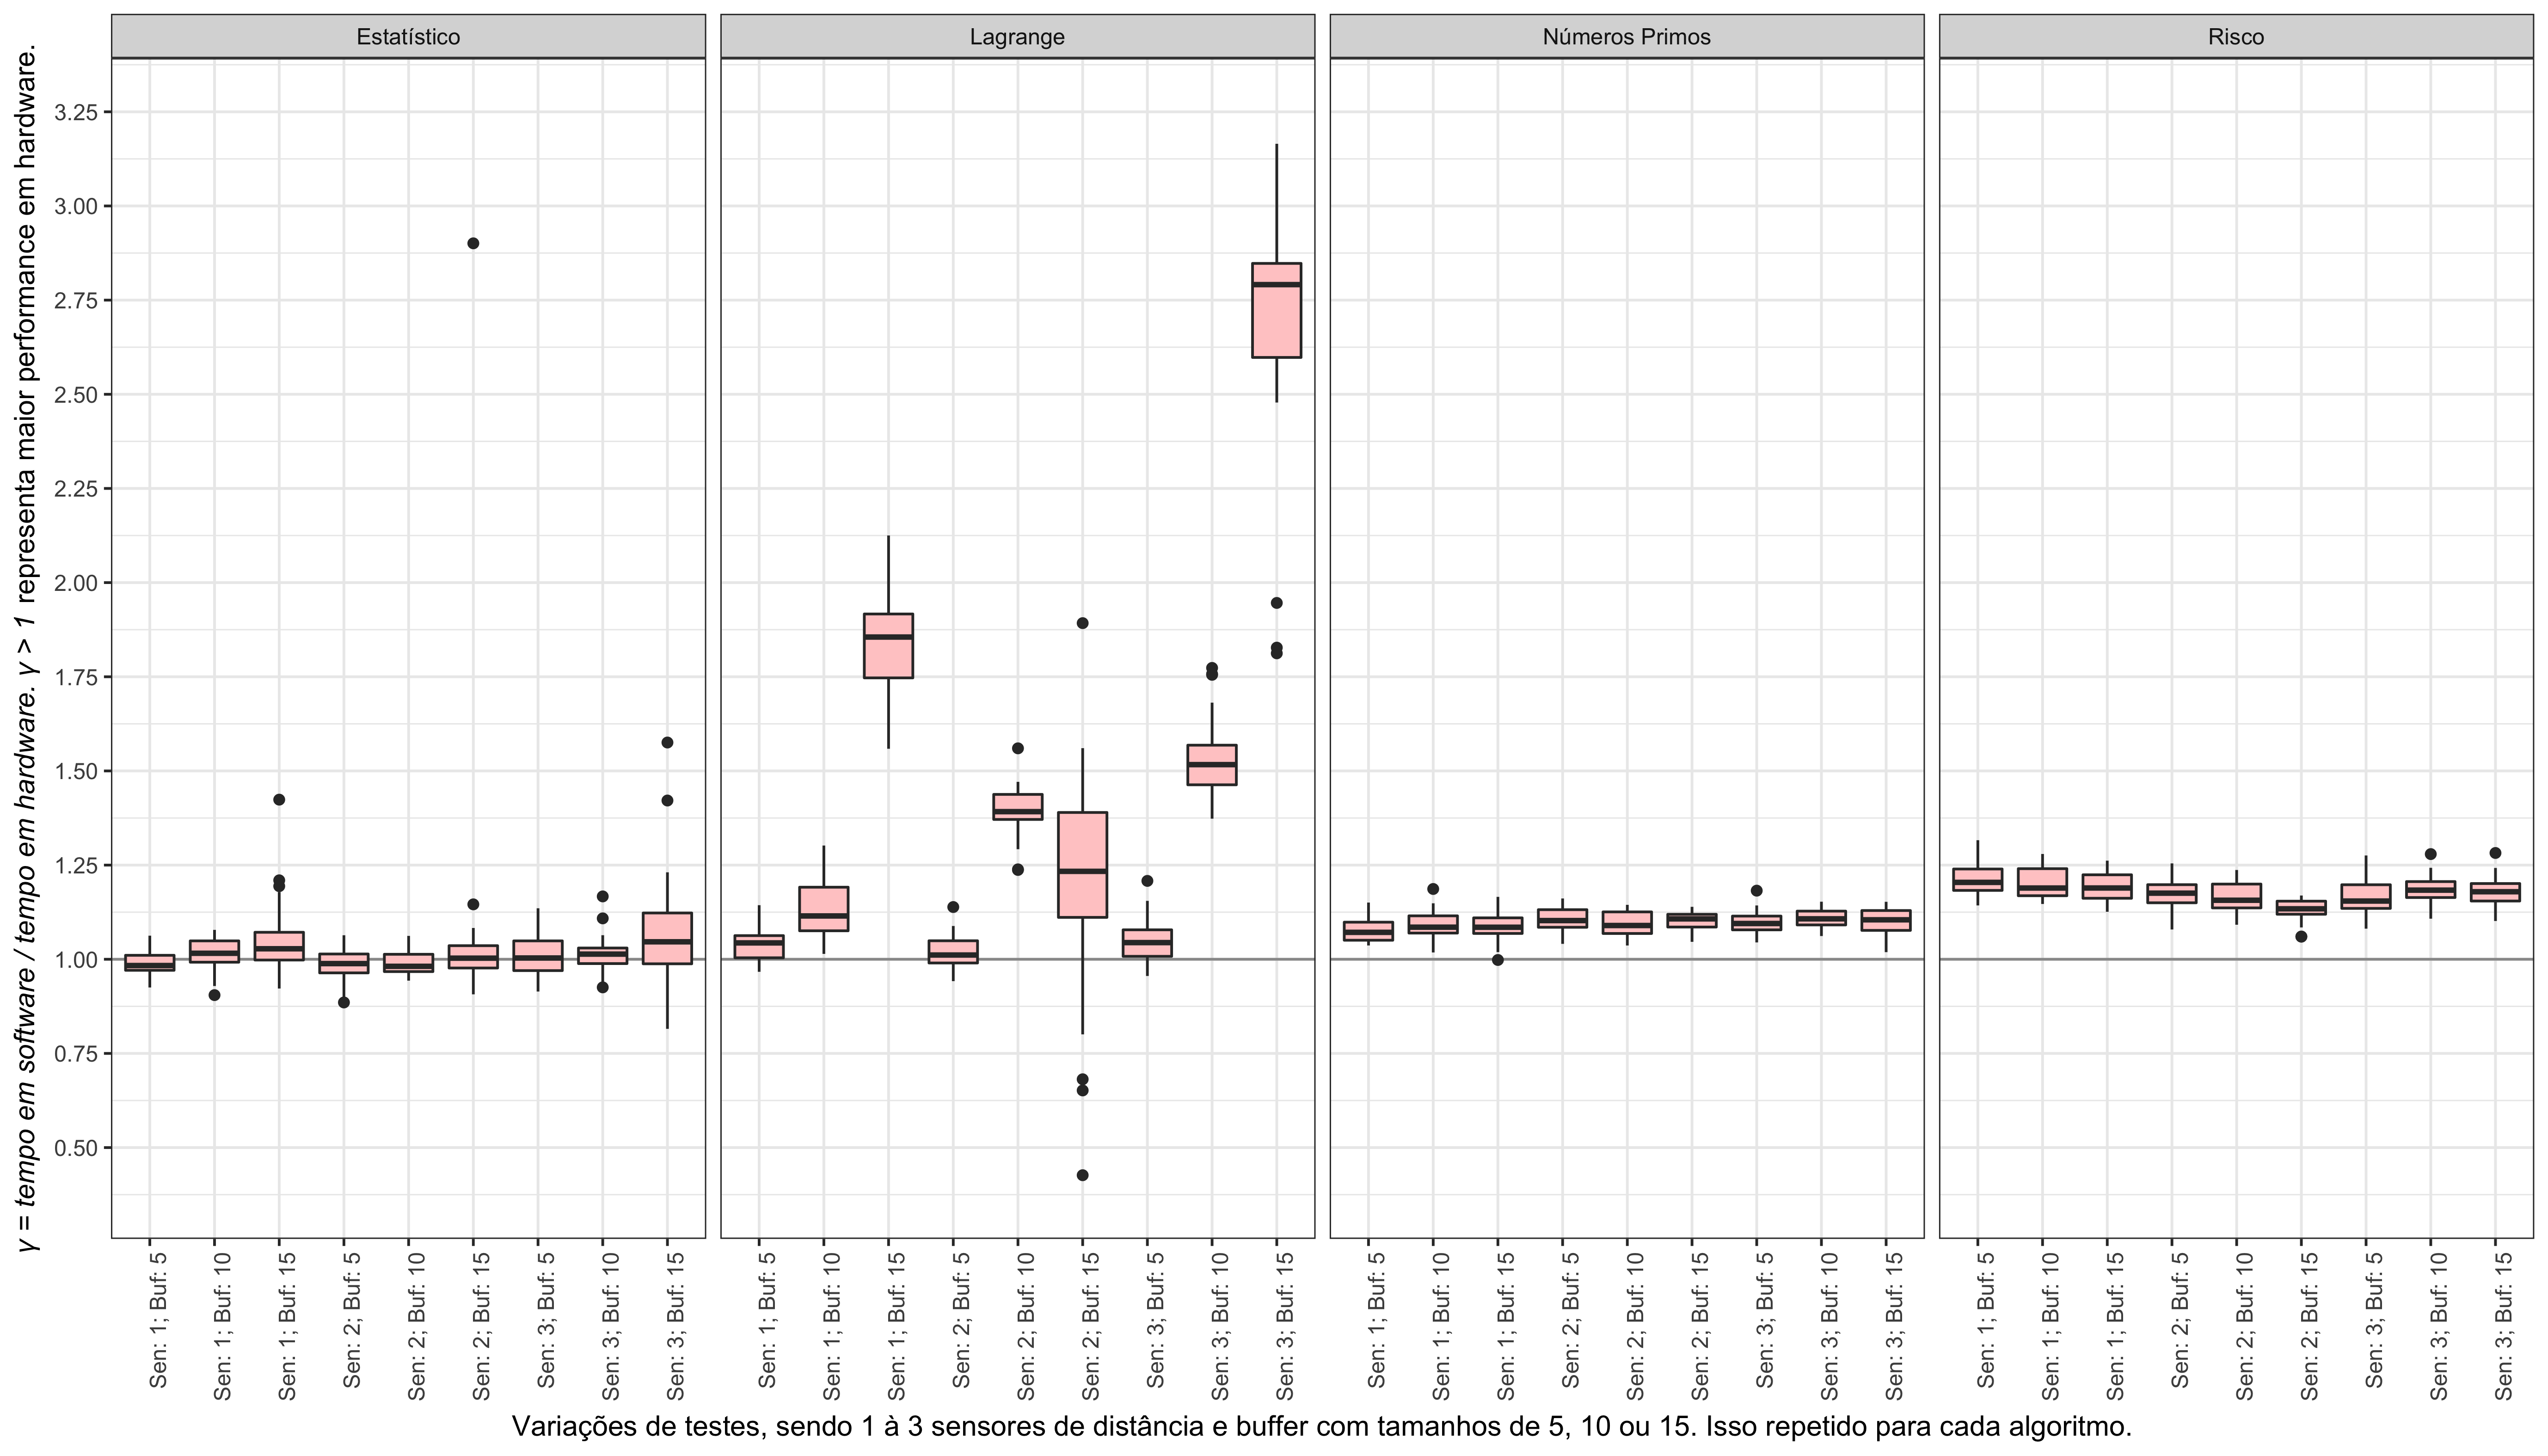
\includegraphics[width=1\textwidth]{img/performance.png}
            \caption{Gráfico com os valores performáticos de cada variação realizada, separados por código particionado. Valores de $\gamma > 1.0 $ exibem maior performance no \hardware\ particionado.}
            \label{fig:performance}
        \end{figure*}
    
        Além da Figura~\ref{fig:performance}, os valores médios de performance entre \software\ e \hardware\ segundo a Seção~\ref{sec:ganho_performance}, também podem ser lidos segundo a Tabela \ref{tab:performance}.
        Cada linha desta Tabela representa um quadro da Figura \ref{fig:performance}.
        Como complemento, na última coluna tem-se uma média de performance geral de cada algoritmo em todas suas variações de teste.
    
        \begin{table}[h]\centering
            \vspace{-1em}
            \scriptsize
            \raaa{1.0}
            %\raaa{0.9}
            \caption{Análise Performática entre os Particionamentos para cada Conjunto de 12 Iterações do Wearable}
            \begin{tabular}{@{}R{1.3em}R{1.6em}R{1.5em}R{1.5em}|R{1.6em}R{1.6em}R{1.6em}|R{1.5em}R{1.5em}R{1.5em}|c@{}}\toprule
                & \multicolumn{3}{c}{1 Sensor} & \multicolumn{3}{c}{2 Sensores} & \multicolumn{3}{c}{3 Sensores}& \\
                \cmidrule{2-11}
                \textit{Buffer} & 5 & 10 & 15 & 5 & 10 & 15 & 5 & 10 & 15 & $\bar{x}$ \\
                \midrule
                \Ss$_{Es}$   & 0.989 & 1.013 & 1.052  & 0.982 & 0.992 & 1.069  & 1.009 & 1.011 & 1.08  & 1.022 \\
                \Ss$_{La}$   & 1.036 & 1.132 & 1.844  & 1.019 & 1.395 & 1.14   & 1.046 & 1.37  & 2.765 & 1.416 \\
                \Ss$_{NP}$   & 1.076 & 1.092 & 1.084  & 1.105 & 1.094 & 1.103  & 1.099 & 1.109 & 1.102 & 1.096 \\ 
                \Ss$_{Ri}$   & 1.212 & 1.203 & 1.195  & 1.17  & 1.161 & 1.132  & 1.168 & 1.183 & 1.179 & 1.178 \\
                \bottomrule
            \end{tabular}
            \label{tab:performance}
        \end{table}
    
        % filtros
        Esses dados receberam filtros das quais eliminou-se: \textit{a):} o tempo médio gasto da atuação dos sensores; bem como \textit{b):} o tempo de envio para o dispositivo externo. 
        O motivo da filtragem é que a performance de ambos dependente diretamente de sua tecnologia e não interferem na performance do particionamento, foco deste documento.
    
    
        %Análise de performance
        % quase todos foram suuuuuuuucesssooooooooo
        Segundos os valores da tabela, percebeu-se que:
        \begin{itemize}
            \item 
            Com esta análise, percebeu-se que os algoritmos Número Primo e Risco (\Ss$_{NP}$ e \Ss$_{Ri}$) obtiveram um ganho de performance considerável e estável comparado com suas versões não particionadas, sendo em média $9,6\%$ e $17,8\%$ mais eficiente em suas tarefas.
            \item 
            Mesmo que o algoritmo Lagrange tenha tido grandes oscilações em seus testes, todos os seus valores médios obtiveram maior performance em \hardware, sendo em média $41,6\%$ mais performático que sua versão em \software.
            \item 
            O algoritmo Estatístico obteve três situações na qual o particionamento em \software\ foi mais performático que em \hardware.
            Entretanto, a média dos valores analisados mostram que ele ainda assim foi $2,2\%$ mais eficiente em \hardware\ que \software;
            \item 
            % Achismos
            O motivo de \Ss$_{Es}$ não ter uma performance maior à \Ss$_{s}$ foi a sua falta de otimização.
            Este algoritmo (Algoritmo \ref{alg:statistic}) é o único que realiza mais de uma leitura sobre os dados de \buffer\ oriundos via parâmetro, sendo as operações situadas nas linhas 4 e 8.
            Este algoritmo como um todo é custoso já que o uso de cada elemento de \buffer\ requer também uma comunicação entre \hs\ solicitando o respectivo dado, criando assim uma sobrecarga de comunicação no barramento e consequentemente a queda de performance.
            %resolvendo o problema
            Uma forma de solução à este problema seria numa otimização utilizando uma memória interna no \hardware\ que, após a cópia de todos os valores do \buffer, pode-se operar lendo da sua própria memória.
            \textit{Pipeline}, \textit{unroll} de \textit{loops} e verificações de dependências de dados são otimizações mais complexas mas que poderiam também resultar em resultados performáticos melhores não só ao algoritmo Estatístico mas também todos os outros;
            \item 
            Nesta pesquisa, utilizou-se de uma única plataforma FPGA para sua realização, partindo de um \textit{soft-}processador para seu fim.
            Com os resultados obtidos, fica visível que seria possível sintetizar esse projeto mesmo em plataformas FPGAs com \luts\ menores que 10 mil caso elas contemplarem com um \textit{hard-}processador.
            Dessa forma, o sistema \wearable\ seria composto de um processador físico e um FPGA, ambos de pequeno porte.
        \end{itemize}
        

\begin{comment}


\begin{table}[h]\centering
\vspace{-1em}
\scriptsize
%\raaa{1.0}
\raaa{0.9}
\caption{Diferença Performática entre os Particionamentos par cada Conjunto de 12 Iterações do Wearable}
\begin{tabular}{@{}R{1.3em}R{1.6em}R{1.5em}R{1.5em}|R{1.6em}R{1.6em}R{1.6em}|R{1.5em}R{1.5em}R{1.5em}|c@{}}\toprule
& \multicolumn{3}{c}{1 Sensor} & \multicolumn{3}{c}{2 Sensores} & \multicolumn{3}{c}{3 Sensores}& \\
\cmidrule{2-11}
\textit{Buf} & 5 & 10 & 15 & 5 & 10 & 15 & 5 & 10 & 15 & $\bar{x}$ \\
\midrule
\Ss$_{Es}$   & -2.0   &    0.5  &    0.4  &   -2.7  &   -1.6  &   -1.8  &    0.4  &   0.3   &     4.2   & -0.2 \\
\Ss$_{La}$   &  7.7   &    9.3  &    8.6  &   10.9  &    9.9  &   11.6  &   10.2  &   12.0  &    12.1   & 10.2 \\
\Ss$_{NP}$   &  2.8   &   12.2  &   91.8  &    1.6  &   44.6  &   13.9  &    4.1  &   64.8  &   231.3   & 51.9 \\
\Ss$_{Ri}$   & 17.8   &   17.2  &   16.9  &   15.0  &   14.9  &   12.9  &   15.0  &   17.5  &    18.4   & 16.1 \\
\bottomrule
\end{tabular}
\label{tab:iterationsmilissegundos}
\end{table}




Power bigger  5,4229934924
Power little  0,7592190889

hls1 ao todo lt 7,7763157895
hls1 ao todo ff 4,4903846154

hls1 ao projeto lt 17,3313782991
hls1 ao projeto ff 14,2813455657

hls2 ao todo lt 8,1677631579
hls2 ao todo ff 4,5769230769

hls2 ao projeto lt 18,3898681677
hls2 ao projeto ff 14,4318957023

maior projeto lut 65,5769230769  ram 18,9791666667      lut all 50,8618421053    ff 31,7139423077             chip
software lut 57,6490384615       ram 18,5520833333      lut all 45,3026315789    ff 27,9134615385             chip

    Expression & Instance      & Multiplexer  & Register & Total
    52 / 0     & 1948 / 1474   & 364 / 0      & 0 / 394   & 2364 / 1868 \\ statistic
    128 / 0    & 2048 / 1425   & 309 / 0      & 0 / 479   & 2483 / 1904 \\ lagrange
    1826 / 0   & 486 / 552     & 236 / 0      & 0 / 527   & 2448 / 1079 \\ prime
    18 / 0     & 120  / 82     & 15  / 0      & 0 / 34    & 153  / 116  \\ risk
    
    
    & LUT    & LUTRAM   & FF     & IO     & On-Chip Power & Power supplied to off-chip devices
    & 20800  & 9600     & 41600  & 210    & -             & - \\
    & 13640  & 1822     & 13080  & 104    & 0,972         & 0,506 \\ statistic
    & 13502  & 1808     & 13193  & 104    & 0,968         & 0,506 \\ lagrange
    & 12959  & 1782     & 12559  & 104    & 0,933         & 0,506 \\ prime
    & 12109  & 1781     & 11742  & 104    & 0,929         & 0,506 \\ risk
    
    (-2,0   +    0,5  +    0,4  +   -2,7  +   -1,6  +   -1,8  +    0,4  +   0,3   +     4,2) / 9 = -0.2
    ( 7,7   +    9,3  +    8,6  +   10,9  +    9,9  +   11,6  +   10,2  +   12,0  +    12,1) / 9 = 10.2
    ( 2,8   +   12,2  +   91,8  +    1,6  +   44,6  +   13,9  +    4,1  +   64,8  +   231,3) / 9 = 51.9
    (17,8   +   17,2  +   16,9  +   15,0  +   14,9  +   12,9  +   15,0  +   17,5  +    18,4) / 9 = 16.1
    
\end{comment}


\begin{comment}
    \begin{table}\centering
    \scriptsize
    \raaa{1.3}
    \caption{Cálculo de performance sobre variações em I/O e algoritmo particionado.}
    \begin{tabular}{@{}rrrrcrrrcrrr@{}}\toprule
    & \multicolumn{3}{c}{$\mathcal{O}(1)$} && \multicolumn{3}{c}{$\mathcal{O}(n)$} & & \multicolumn{3}{c}{$\mathcal{O}(n\log n)$}\\
    \cmidrule{2-4} \cmidrule{6-8} \cmidrule{10-12}análise& 5 & 10 & 15 && 5 & 10 & 15 &&5 & 10 & 15 \\
    \midrule \textit{sistêmica} \\
    %média     & ? & ? & ? && ? & ? & ? && ? & ? & ? \\
    $\bar{x}$     & ? & ? & ? && ? & ? & ? && ? & ? & ? \\
    $\sigma^2$ & ? & ? & ? && ? & ? & ? && ? & ? & ? \\
    $\sigma$ & ? & ? & ? && ? & ? & ? && ? & ? & ? \\
    \midrule \textit{empírica} \\
    %média     & ? & ? & ? && ? & ? & ? && ? & ? & ? \\
    $\bar{x}$     & ? & ? & ? && ? & ? & ? && ? & ? & ? \\
    $\sigma^2$ & ? & ? & ? && ? & ? & ? && ? & ? & ? \\
    $\sigma$ & ? & ? & ? && ? & ? & ? && ? & ? & ? \\
    \bottomrule
    \end{tabular}
    \end{table}
    \end{frame}
\end{comment}

